\documentclass[conference]{IEEEtran}
\IEEEoverridecommandlockouts
% The preceding line is only needed to identify funding in the first footnote. If that is unneeded, please comment it out.
\usepackage{cite}
\usepackage{amsmath,amssymb,amsfonts}
\usepackage{algorithmic}
\usepackage{graphicx}
\usepackage{textcomp}
\usepackage{xcolor}
\usepackage{hyperref}
\usepackage{subfig}

\def\BibTeX{{\rm B\kern-.05em{\sc i\kern-.025em b}\kern-.08em
    T\kern-.1667em\lower.7ex\hbox{E}\kern-.125emX}}
\begin{document}

\title{Model Driven Approach for Migration Problem in Hybrid App Development\\}

%TODO: Insert names for each team member%
\author{\IEEEauthorblockN{1\textsuperscript{st} Given Name Surname}
\IEEEauthorblockA{\textit{dept. name of organization (of Aff.)} \\
\textit{name of organization (of Aff.)}\\
City, Country \\
email address or ORCID}
\and
\IEEEauthorblockN{2\textsuperscript{nd} Given Name Surname}
\IEEEauthorblockA{\textit{dept. name of organization (of Aff.)} \\
\textit{name of organization (of Aff.)}\\
City, Country \\
email address or ORCID}
\and
\IEEEauthorblockN{Riordan Dervin Alfredo}
\IEEEauthorblockA{\textit{Faculty of IT, Monash University} \\
Melbourne, Australia \\
riordan.alfredo@gmail.com}
\and
\IEEEauthorblockN{ Raymond Nguyen }
\IEEEauthorblockA{\textit{Faculty of IT} \\
\textit{Monash University}\\
Melbourne, Australia \\
rmngu2@student.monash.edu}
}

\maketitle

\begin{abstract}
Software migration is a common problem for developers working in industry or even working on personal projects. It is usually time consuming
and difficult to test if it has been done correctly. Nowadays may web application frameworks have different versions which makes it difficult
to migrate given how frequently they change. One key example is the Ionic Framework which is used to help build desktop as well as mobile applications,
with a simple "write once, deploy anywhere" type of strategy. The Ionic Framework has a manual migration guide that can help developers migrate from 
different versions, however we proposed a model-driven apporach to aid the migration process. By focusing on a model-driven approach, we can develop a model
which is a representation of the system which will generate code for a specific version. Our approach was applied to a case study in order to validate
whether this approach was successful or not. 
\end{abstract}

\section{Introduction}
At some point in the software lifecycle, the current system must be migrated into a new system or version. 
Software migration is the intricate process of moving an application from one environment or version to another. 
Software migration in general, usually consumes lots of resources, time, and effort. 
\\ According to the online article (IBM, 2014) \cite{b1}, it described several common challenges in migrating software applications. In terms of business aspects, these include: determining when to migrate, resistance of users culture and the migration itself not being completed on time. 
For the technical aspects, these include: minimizing disruption of mission critical applications and ensuring that the application functions correctly after migration.
\\ These migration challenges are common for new technologies, especially for web and mobile-based applications as they are constantly changing. Recently, hybrid apps have become popular as an alternative to native mobile applications. Hybrid applications host a web application inside a 
native webview while utilizing bridges that allow access to native app functions such as camera access, geolocation, etc. 
This means that developers are able to carry over their expertise with web technologies to mobile app development without needing to learn native tech stacks. 
\\ A key example of this is the Ionic Framework which is a very popular hybrid application development framework that employs a ‘write once, deploy anywhere’ approach. The latest version of Ionic (version 4) was 
a complete rewrite that makes it incompatible with projects written in Ionic 3, which makes it a suitable candidate for the research project.
\\ There are several differences between Ionic 3 and 4, which makes it worth the port, including compatibility with any front-end framework as opposed to Ionic 3’s tight coupling with Angular. 
There are quite a few issues that can deter development teams from doing a manual port to Ionic 4 which includes breaking changes to the library versions used in both framework versions. Despite there being a guide into how to manually migrate from an Ionic 3 project to an Ionic 4 project, 
there are still a vast number of forums dedicated to help solve the manual migration process. 
\\ One potential solution to solve these problems is to create models to help generate code to support the migration process. 
This might be achieved with a software engineering technique called model-driven development. Model-driven approaches are used mainly in software design to generally 
simplify a complex process of the system into a higher-level abstraction. By abstracting the migration process into a code generation tool, it could possibly speed up the 
migration process with high accuracy and consistency as intended. In addition, it would benefit developers as it is a more efficient way to deal with the migration problems.
\\ Finally, applying a model driven approach would not just be applicable to the Ionic framework, but potentially other web frameworks as well. 
Therefore, model-driven approaches might solve software migration problems towards hybrid app development in regards to technical and business aspects 
that industry is currently facing. Using a model-driven approach as well as focusing on Ionic versions 3 and 4, the research undertaken will determine whether 
the issue of model driven approaches for migration can be applied.
\newline \newline Looking into the problem a bit more, we have devised a main research question below.
\newline \newline \textbf{Can model-driven development provide a valid migration solution?}
\newline \newline Branching away from this primary question, we can ask further questions that target specific concerns about the migration tool we are proposing to create using model-driven development:
\begin{enumerate}
    \item Can it account for major changes like different libraries/versions?
    \newline Looking at the Ionic Framework, there are specific libraries or versions used in a project that may differ from one version to another. 
    These may involve small changes like simply changing the name to match the new version or larger changes such as changing the way the application handles routing to different pages. 
    Our research will involve taking a look at some of these changes.
    \item Is generated code of acceptable quality?
    \newline With the model being used to help convert one Ionic 3 project file to a compatible Ionic 4 version, there can be a chance that the migration may not be perfect. 
    There might be flaws with the output of the conversion which breaks the integrity of the original file. Our research will also observe the quality of the code and take note of any changes.
    \item Can the tool be used for other case studies?
    \newline Our modelling tool will be primarily used for our case study (Meetup For Pets) however every Ionic project is expected to be different. 
    Our research will observe to see if the tool will be applicable not just for our case study, but for other Ionic 3 projects as well. 
\end{enumerate}
The contributions of this work are as follows:
\begin{itemize}
    \item We will introduce a case study Ionic 3 application (MeetUp For Pets) built primarily to test the viability of a proposed model
    \item A metamodel will be built as well as a model which performs code generation to convert from Ionic 3 to Ionic 4
    \item Our findings and evaluations will then be presented on the feasibility of using a model driven approach for migrating using the Ionic Framework as the primary focus
\end{itemize}

\section{Approach}

\subsection{Case Study}
As a proof-of-concept, the application that will be developed for our case study will be called \textbf{Meetups for Pets}. It is a hybrid application written 
in Ionic version 3 to connect pet enthusiasts to promote face-to-face interactions with pets and their owners. The users will have the ability to organise a 
meetups with each pet’s owner. The main purpose of this case study is to test the model-driven migration tool, this can be shown in \ref{fig:meetupIonic}
\begin{figure}%
    \centering
    \subfloat[The home page of Meetup for Pets]{{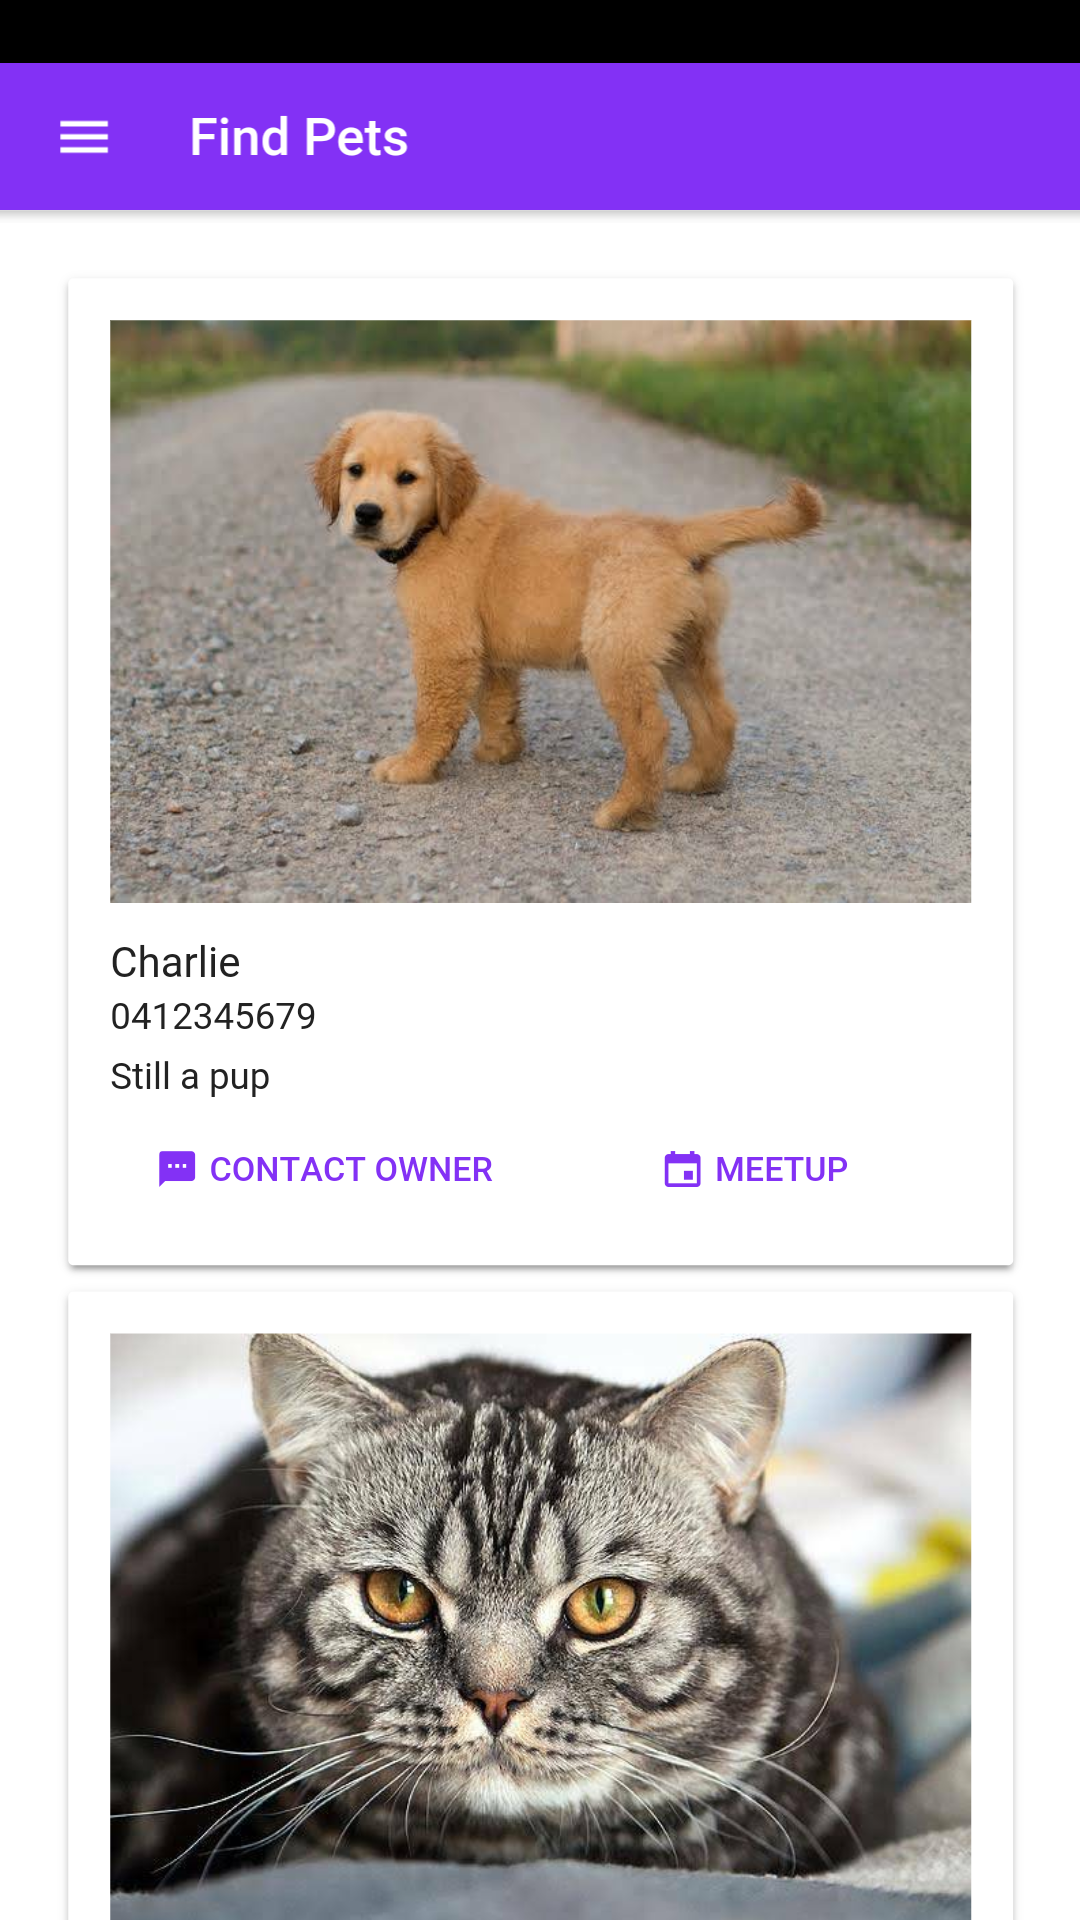
\includegraphics[scale=0.1]{find_pets.png} }}%
    \qquad
    \subfloat[A list of pets that a user owns]{{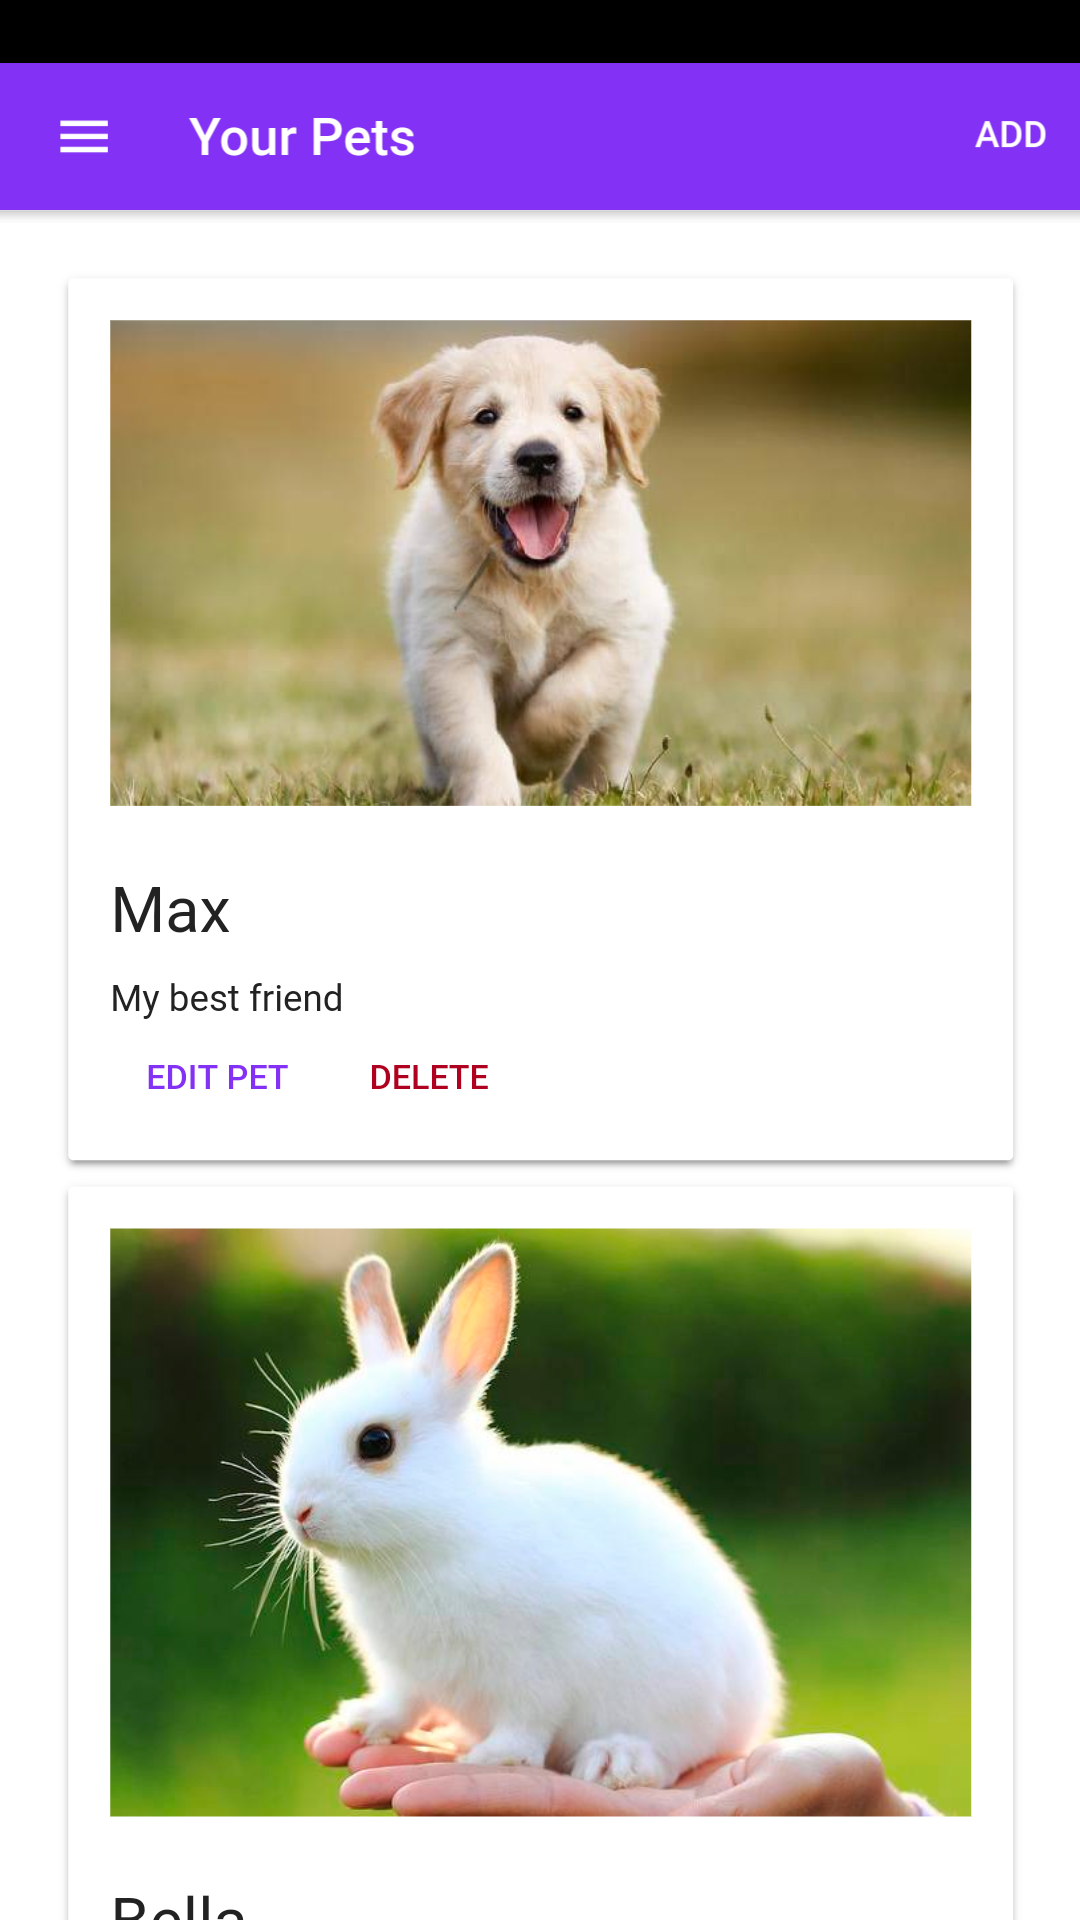
\includegraphics[scale=0.1]{your_pets.png} }}%
    \caption{Meetup For Pets Ionic 3 Application}%
    \label{fig:meetupIonic}%
\end{figure}
\\ In a real-world scenario, an application would normally take advantage of the hardware capabilities of the device it is running on. 
Therefore, there are some Ionic native framework features that were included, such as camera, contacts, calendar, and messaging.
\\ Using the case study above, we attempted to perform some manual migration to look deeper into the issues that may arise when migrating. 


\subsection{The Modelling Tool}
\section{Evaluation}
Before you begin to format your paper, first write and save the content as a 
separate text file. Complete all content and organizational editing before 
formatting. Please note sections \ref{AA}--\ref{SCM} below for more information on 
proofreading, spelling and grammar.

Keep your text and graphic files separate until after the text has been 
formatted and styled. Do not number text heads---{\LaTeX} will do that 
for you.

\subsection{Abbreviations and Acronyms}\label{AA}
Define abbreviations and acronyms the first time they are used in the text, 
even after they have been defined in the abstract. Abbreviations such as 
IEEE, SI, MKS, CGS, ac, dc, and rms do not have to be defined. Do not use 
abbreviations in the title or heads unless they are unavoidable.

\subsection{Units}
\begin{itemize}
\item Use either SI (MKS) or CGS as primary units. (SI units are encouraged.) English units may be used as secondary units (in parentheses). An exception would be the use of English units as identifiers in trade, such as ``3.5-inch disk drive''.
\item Avoid combining SI and CGS units, such as current in amperes and magnetic field in oersteds. This often leads to confusion because equations do not balance dimensionally. If you must use mixed units, clearly state the units for each quantity that you use in an equation.
\item Do not mix complete spellings and abbreviations of units: ``Wb/m\textsuperscript{2}'' or ``webers per square meter'', not ``webers/m\textsuperscript{2}''. Spell out units when they appear in text: ``. . . a few henries'', not ``. . . a few H''.
\item Use a zero before decimal points: ``0.25'', not ``.25''. Use ``cm\textsuperscript{3}'', not ``cc''.)
\end{itemize}

\section{Discussion/Experiences}
Number equations consecutively. To make your 
equations more compact, you may use the solidus (~/~), the exp function, or 
appropriate exponents. Italicize Roman symbols for quantities and variables, 
but not Greek symbols. Use a long dash rather than a hyphen for a minus 
sign. Punctuate equations with commas or periods when they are part of a 
sentence, as in:
\begin{equation}
a+b=\gamma\label{eq}
\end{equation}

Be sure that the 
symbols in your equation have been defined before or immediately following 
the equation. Use ``\eqref{eq}'', not ``Eq.~\eqref{eq}'' or ``equation \eqref{eq}'', except at 
the beginning of a sentence: ``Equation \eqref{eq} is . . .''


\section{Related Work}
Number equations consecutively. To make your 
equations more compact, you may use the solidus (~/~), the exp function, or 
appropriate exponents. Italicize Roman symbols for quantities and variables, 
but not Greek symbols. Use a long dash rather than a hyphen for a minus 
sign. Punctuate equations with commas or periods when they are part of a 
sentence, as in:
\begin{equation}
a+b=\gamma\label{eq}
\end{equation}

Be sure that the 
symbols in your equation have been defined before or immediately following 
the equation. Use ``\eqref{eq}'', not ``Eq.~\eqref{eq}'' or ``equation \eqref{eq}'', except at 
the beginning of a sentence: ``Equation \eqref{eq} is . . .''


\section{Conclusion}
Number equations consecutively. To make your 
equations more compact, you may use the solidus (~/~), the exp function, or 
appropriate exponents. Italicize Roman symbols for quantities and variables, 
but not Greek symbols. Use a long dash rather than a hyphen for a minus 
sign. Punctuate equations with commas or periods when they are part of a 
sentence, as in:
\begin{equation}
a+b=\gamma\label{eq}
\end{equation}

Be sure that the 
symbols in your equation have been defined before or immediately following 
the equation. Use ``\eqref{eq}'', not ``Eq.~\eqref{eq}'' or ``equation \eqref{eq}'', except at 
the beginning of a sentence: ``Equation \eqref{eq} is . . .''

\subsection{\LaTeX-Specific Advice}

Please use ``soft'' (e.g., \verb|\eqref{Eq}|) cross references instead
of ``hard'' references (e.g., \verb|(1)|). That will make it possible
to combine sections, add equations, or change the order of figures or
citations without having to go through the file line by line.

Please don't use the \verb|{eqnarray}| equation environment. Use
\verb|{align}| or \verb|{IEEEeqnarray}| instead. The \verb|{eqnarray}|
environment leaves unsightly spaces around relation symbols.

Please note that the \verb|{subequations}| environment in {\LaTeX}
will increment the main equation counter even when there are no
equation numbers displayed. If you forget that, you might write an
article in which the equation numbers skip from (17) to (20), causing
the copy editors to wonder if you've discovered a new method of
counting.

{\BibTeX} does not work by magic. It doesn't get the bibliographic
data from thin air but from .bib files. If you use {\BibTeX} to produce a
bibliography you must send the .bib files. 

{\LaTeX} can't read your mind. If you assign the same label to a
subsubsection and a table, you might find that Table I has been cross
referenced as Table IV-B3. 

{\LaTeX} does not have precognitive abilities. If you put a
\verb|\label| command before the command that updates the counter it's
supposed to be using, the label will pick up the last counter to be
cross referenced instead. In particular, a \verb|\label| command
should not go before the caption of a figure or a table.

Do not use \verb|\nonumber| inside the \verb|{array}| environment. It
will not stop equation numbers inside \verb|{array}| (there won't be
any anyway) and it might stop a wanted equation number in the
surrounding equation.

\subsection{Some Common Mistakes}\label{SCM}
\begin{itemize}
\item The word ``data'' is plural, not singular.
\item The subscript for the permeability of vacuum $\mu_{0}$, and other common scientific constants, is zero with subscript formatting, not a lowercase letter ``o''.
\item In American English, commas, semicolons, periods, question and exclamation marks are located within quotation marks only when a complete thought or name is cited, such as a title or full quotation. When quotation marks are used, instead of a bold or italic typeface, to highlight a word or phrase, punctuation should appear outside of the quotation marks. A parenthetical phrase or statement at the end of a sentence is punctuated outside of the closing parenthesis (like this). (A parenthetical sentence is punctuated within the parentheses.)
\item A graph within a graph is an ``inset'', not an ``insert''. The word alternatively is preferred to the word ``alternately'' (unless you really mean something that alternates).
\item Do not use the word ``essentially'' to mean ``approximately'' or ``effectively''.
\item In your paper title, if the words ``that uses'' can accurately replace the word ``using'', capitalize the ``u''; if not, keep using lower-cased.
\item Be aware of the different meanings of the homophones ``affect'' and ``effect'', ``complement'' and ``compliment'', ``discreet'' and ``discrete'', ``principal'' and ``principle''.
\item Do not confuse ``imply'' and ``infer''.
\item The prefix ``non'' is not a word; it should be joined to the word it modifies, usually without a hyphen.
\item There is no period after the ``et'' in the Latin abbreviation ``et al.''.
\item The abbreviation ``i.e.'' means ``that is'', and the abbreviation ``e.g.'' means ``for example''.
\end{itemize}
An excellent style manual for science writers is \cite{b7}.

\subsection{Authors and Affiliations}
\textbf{The class file is designed for, but not limited to, six authors.} A 
minimum of one author is required for all conference articles. Author names 
should be listed starting from left to right and then moving down to the 
next line. This is the author sequence that will be used in future citations 
and by indexing services. Names should not be listed in columns nor group by 
affiliation. Please keep your affiliations as succinct as possible (for 
example, do not differentiate among departments of the same organization).

\subsection{Identify the Headings}
Headings, or heads, are organizational devices that guide the reader through 
your paper. There are two types: component heads and text heads.

Component heads identify the different components of your paper and are not 
topically subordinate to each other. Examples include Acknowledgments and 
References and, for these, the correct style to use is ``Heading 5''. Use 
``figure caption'' for your Figure captions, and ``table head'' for your 
table title. Run-in heads, such as ``Abstract'', will require you to apply a 
style (in this case, italic) in addition to the style provided by the drop 
down menu to differentiate the head from the text.

Text heads organize the topics on a relational, hierarchical basis. For 
example, the paper title is the primary text head because all subsequent 
material relates and elaborates on this one topic. If there are two or more 
sub-topics, the next level head (uppercase Roman numerals) should be used 
and, conversely, if there are not at least two sub-topics, then no subheads 
should be introduced.

\subsection{Figures and Tables}
\paragraph{Positioning Figures and Tables} Place figures and tables at the top and 
bottom of columns. Avoid placing them in the middle of columns. Large 
figures and tables may span across both columns. Figure captions should be 
below the figures; table heads should appear above the tables. Insert 
figures and tables after they are cited in the text. Use the abbreviation 
``Fig.~\ref{fig}'', even at the beginning of a sentence.
% Below is the method to create a table %
\begin{table}[htbp]
\caption{Table Type Styles}
\begin{center}
\begin{tabular}{|c|c|c|c|}
\hline
\textbf{Table}&\multicolumn{3}{|c|}{\textbf{Table Column Head}} \\
\cline{2-4} 
\textbf{Head} & \textbf{\textit{Table column 1}}& \textbf{\textit{Subhead}}& \textbf{\textit{Subhead}} \\
\hline
copy& More table copy$^{\mathrm{a}}$& &  \\
\hline
\multicolumn{4}{l}{$^{\mathrm{a}}$Sample of a Table footnote.}
\end{tabular}
\label{tab1}
\end{center}
\end{table}

\begin{figure}[htbp]
\centerline{
\includegraphics{fig1.png}}
\caption{Example of a figure caption.}
\label{fig}
\end{figure}

Figure Labels: Use 8 point Times New Roman for Figure labels. Use words 
rather than symbols or abbreviations when writing Figure axis labels to 
avoid confusing the reader. As an example, write the quantity 
``Magnetization'', or ``Magnetization, M'', not just ``M''. If including 
units in the label, present them within parentheses. Do not label axes only 
with units. In the example, write ``Magnetization (A/m)'' or ``Magnetization 
\{A[m(1)]\}'', not just ``A/m''. Do not label axes with a ratio of 
quantities and units. For example, write ``Temperature (K)'', not 
``Temperature/K''.

\section*{Acknowledgment}

The preferred spelling of the word ``acknowledgment'' in America is without 
an ``e'' after the ``g''. Avoid the stilted expression ``one of us (R. B. 
G.) thanks $\ldots$''. Instead, try ``R. B. G. thanks$\ldots$''. Put sponsor 
acknowledgments in the unnumbered footnote on the first page. 
\section*{References}

Please number citations consecutively within brackets \cite{b1}. The 
sentence punctuation follows the bracket \cite{b2}. Refer simply to the reference 
number, as in \cite{b3}---do not use ``Ref. \cite{b3}'' or ``reference \cite{b3}'' except at 
the beginning of a sentence: ``Reference \cite{b3} was the first $\ldots$''

Number footnotes separately in superscripts. Place the actual footnote at 
the bottom of the column in which it was cited. Do not put footnotes in the 
abstract or reference list. Use letters for table footnotes.

Unless there are six authors or more give all authors' names; do not use 
``et al.''. Papers that have not been published, even if they have been 
submitted for publication, should be cited as ``unpublished'' \cite{b4}. Papers 
that have been accepted for publication should be cited as ``in press'' \cite{b5}. 
Capitalize only the first word in a paper title, except for proper nouns and 
element symbols.

For papers published in translation journals, please give the English 
citation first, followed by the original foreign-language citation \cite{b6}.

% @Author: Riordan Dervin Alfredo, 2/11/2019 %
\section{Related Work}
In regards to the software migration that utilises model driven engineering methods,
there are already several studies that were conducted extensively before.
Those are; FASMM: 
Fast and Accessible Software Migration Method \cite{b9}, Reverse Engineering 
Strategies for Software Migration \cite{b10}, Model-Driven Engineering 
for Software Migration in a Large Industrial Context \cite{b11},  
Towards a Model-Driven Approach for Planning a 
Standard-Based Migration of Enterprise Applications to SOA  \cite{b12}, and
Migrating C/C++ Software to Mobile Platforms in the ADM Context \cite{b8}

Our study is closely related to the FASMM approaches \cite{b9} as this research
provides extensive guides for software developers that have limited 
resources (time, budget, workforce $\ldots$) to conduct software migration. 
\cite{b10} study provides specific methods to conduct reverse-engineering 
that is involved our process.

In \cite{b11} and \cite{b12} studies are proving the feasibility of model-driven engineering
in diffent domain and contexts from our studies. Those are the migration to another completely new framework, 
migration to a new architecture (legacy achitecture to service-oriented architecture), and migration
of different languages to specific mobile applications framework. 
They also provided insights of how model-driven engineering processes to be economically
profitable and provides cost-effectiveness. 

The \cite{b8} study related to our work in terms of processing different kind of 
programming languages and paradigms to generate mobile application codes. It is also 
the main example of feasibility model-driven in the software migration of mobile applications,
which is in our case is software migration of the hybrid mobile application.

Each related work are explained in details below,

\textcolor{red}{ if it is too much, I can remove this section below}

\subsection{ FASMM: Fast and Accessible Software Migration Method }
\textcolor{blue}{<draft>}

\subsection{ Model-Driven Engineering for Software Migration in a Large Industrial Context }
This paper describes the process of migrating a large-scale software application from Mainframe to J2EE
using Model-Driven Engineering process. The migration process in this study starts by describing the general 
processes of current legacy system.

First, a parser is created to make an abstract systax tree from the legacy code. Then, it is processed
by a transformation to build a model that conforms to the meta-model of the legacy language.
During the second stage, all symbols are resolved and bound to appropriate model elements.

Afterwards, from code model, reverse-engineering process is conducted to produce a platform independent 
model. Finally, this model will be mapped into a platform specific model that can be used to generate code
for the final product of the migrated application. 

\subsection{ Towards a Model-Driven Approach for Planning a Standard-Based Migration of Enterprise Applications to SOA }
\textcolor{blue}{<draft>}

\subsection{ Migrating C/C++ Software to Mobile Platforms in the ADM Context }
This study took an example of  C/C++ language to produce Android, IoS, and Windows mobile application. 
In our study, the extension type of generated codes are still maintained,
but the main code-generation process is technically alike . 

Furthermore, this study gives insight in regards to feasibility of model-driven development approach that is 
advanced to ADM (Architecture-Driven Modernization) within similar domain, mobile application migration. 
ADM approach that are described in this study could potentially be part of the future works in our study. 
The validation tool that is used in this research is to our approach, which is Eclipse Modeling Framework.
mobile applications from different kind of programming languages, which is technically 
how hybrid application system or architecture works. 

\section{Conclusion}
In conclusion, our study contributes in the success and feasibility for another area 
of software migration with model-driven engineering methodologies, which is hybrid application domain.
At this stage, our approaches only prove small fraction of hybrid application domain because 
this study only focused only at one framework (Ionic) and selected specific versions (migrating version 3 to version 4). 

At the moment, within these constraints, the tool that we had created only handle basics migration functionalities.
Basically, this migration tool is only using string parser, transformation, and code-generation. These process might
be insufficient to handle more complex functionalities as described in our limitations.

There are still many other challenges to tackle in the proposed methods to fully migrate the Ionic version 3 project
to version 4. This is due to our proposed approach is still in the feasibility study to fully migrate the hybrid application 
completely. Despite all of these challenges and limitations, our approach could potentitally open-up path for further research
in the software migration of hybrid application by utilising model-driven engineering approaches.  

\section{Future Work}
Here, we used the Eclipse Modeling Framework as our validator and main tool to migrate the Ionic framework 
from version 3 to version 4. Within this tool, the abstraction level is intentionally increased for the 
cohesiveness and extensibility of migration functions, while correspondingly reduce couplings between 
functions. Future researchers could upgrade more complex functionalities based on the limitations that 
we had listed above.

The main reason is the tool that we had created was only able solving basic migration problems. 
It requires more extensive research to solve more complex functionalites, such as dealing with 
architectural level to arrange files in correct directories position. The potential
higher-level model-driven approach that could possibly be exercised is ADM (Architecture-Driven Modernization) \cite{b8}. 

There will be time in the future for this tool to be mature that could migrate Ionic Framework application from version 
3 to version 4 thoroughly, without introducing any migration bugs.
This tool is also envisioned to handle migration of Ionic framework from 
any versions to the latest. In the further future, by following our approaches and further research, 
it could potentially able to migrate other different hybrid application frameworks' versions.

\begin{thebibliography}{00}
\bibitem{b1} IBM (2014). Challenges when migrating applications. Retrieved 7 September 2019, from \url{https://www.ibm.com/support/knowledgecenter/en/SSEP7J_10.2.1/com.ibm.swg.ba.cognos.ug_mfdm.10.2.1.doc/c_mfdm_chal_mig.html}
\bibitem{b2} J. Clerk Maxwell, A Treatise on Electricity and Magnetism, 3rd ed., vol. 2. Oxford: Clarendon, 1892, pp.68--73.
\bibitem{b3} I. S. Jacobs and C. P. Bean, ``Fine particles, thin films and exchange anisotropy,'' in Magnetism, vol. III, G. T. Rado and H. Suhl, Eds. New York: Academic, 1963, pp. 271--350.
\bibitem{b4} K. Elissa, ``Title of paper if known,'' unpublished.
\bibitem{b5} R. Nicole, ``Title of paper with only first word capitalized,'' J. Name Stand. Abbrev., in press.
\bibitem{b6} Y. Yorozu, M. Hirano, K. Oka, and Y. Tagawa, ``Electron spectroscopy studies on magneto-optical media and plastic substrate interface,'' IEEE Transl. J. Magn. Japan, vol. 2, pp. 740--741, August 1987 [Digests 9th Annual Conf. Magnetics Japan, p. 301, 1982].
\bibitem{b7} M. Young, The Technical Writer's Handbook. Mill Valley, CA: University Science, 1989.

% Related works' biblioraphies %
\bibitem{b8} Martinez, L., et al. ``Migrating C/C++ Software to Mobile Platforms in the ADM context,'' \textit{International Journal of Interactive Multimedia and Artificial Intelligence}, Vol. 4 , N\textsuperscript{o}3, p. 34, 2017. [Abstract]. Available: Semantics Scholar, URL: \url{https://pdfs.semanticscholar.org/8968/7958518252817c4bbe02c77fcef5a48a8d3c.pdf}, [Accessed November 1, 2019].
\bibitem{b9} Forite, L. and C. Hug. ``FASMM: Fast and Accessible Software Migration Method,'' in Research Challenges in Information Science (RCIS), 2014 IEEE Eights Internation Conference on. 2014, IEEE.
\bibitem{b10} Muller, H. A. ``Reverse Engineering Strategies for Software Migration'', in Proceedings of the (19\textsuperscript{th}) International Conference on Software Engineering, May 1997, p. 659, IEEE.
\bibitem{b11} Fleurey, F., et al. ``Model-Driven Engineering for Software Migration in a Large Industrial Context'', in International Conference on Model Driven Engineering Languages and Systems, 2007, pp. 482-497, MODELS
\bibitem{b12} Aboulsamh, M.A. ``Towards a Model-Driven Approach for Planning a Standard-Based Migration of Enterprise Applications to SOA'', in 2009 Congress on Services - l , 2009, IEEE.

\end{thebibliography}
\vspace{12pt}
\color{red}

\end{document}
